\documentclass[10pt, a4paper]{article}

\usepackage{amsmath}
\usepackage{amssymb}
\usepackage{fullpage}
\usepackage{algorithm2e}
\usepackage{graphicx}
\usepackage{wrapfig}



\newcounter{wssection}
\newcounter{wsexercise}[wssection]


\newcommand{\worksheetsection}[1]{
\vspace{10mm}
\stepcounter{wssection}
\noindent \Large \textbf{\thewssection. #1} \normalsize
\vspace{3mm}
}


\newcommand{\worksheetexercise}{
\stepcounter{wsexercise}
\vspace{5mm} \noindent \textbf{Exercise \thewssection.\thewsexercise \;}
}


\title{Dublin R Workshop on Time Series Analysis}
\author{Mick Cooney\\mickcooney@gmail.com}
\date{Autumn 2013}



\begin{document}

\maketitle



%%%
%%% SECTION: Basic Concepts
%%%

\worksheetsection{Basic Concepts}

\noindent
Time series occur in almost any field of study that produces
quantitative data. Whenever quantities are measured over time, those
measurements form a time-series, or more formally, a
\emph{discrete-time stochastic process}.

One reasonably famous example of a time-series is count of airline
passengers in the US, as seen in Figure \ref{fig1}. This is a fairly
simple time-series, with measurements taken on a monthly basis over a
number of years, with each datum consisting of a single number,
i.e. this time-series is \emph{univariate}.

\begin{figure}[h]
\begin{center}
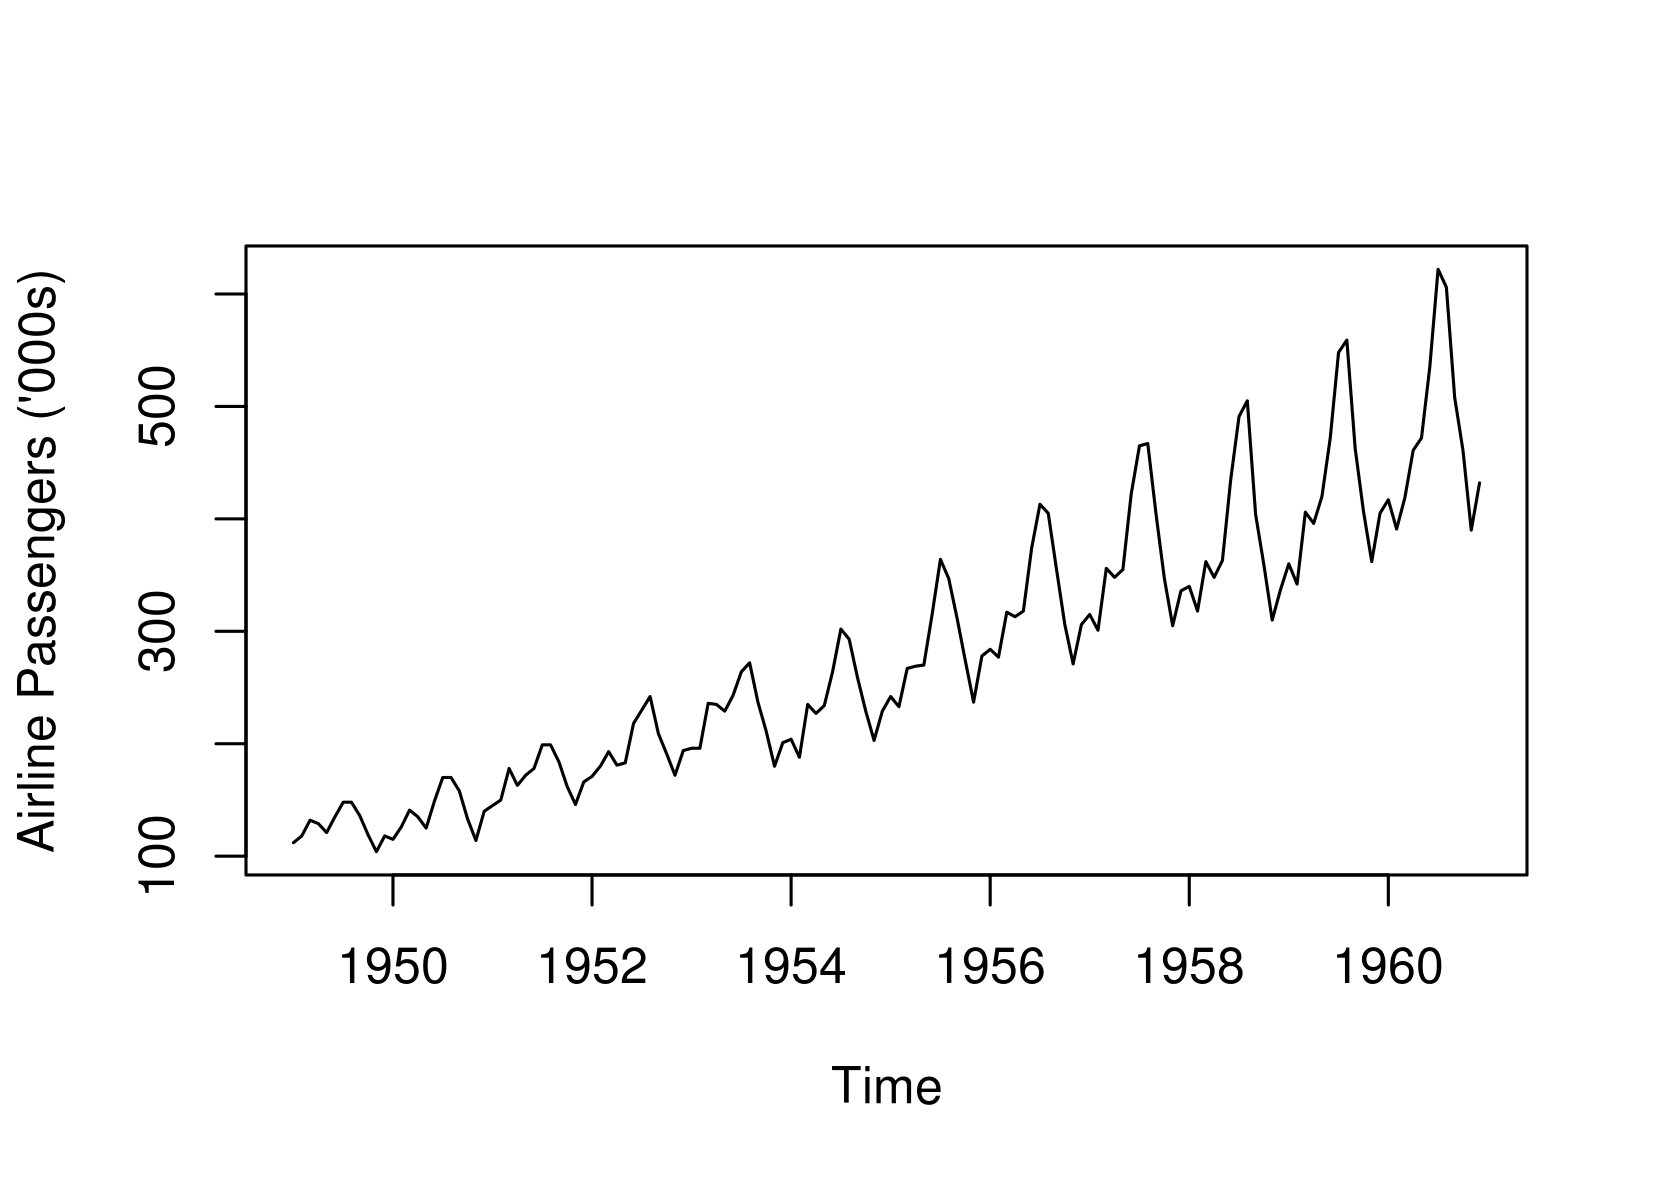
\includegraphics{airline_passengers_plot.png}
\caption{\label{fig1}
Example of a Time Series: Monthly Airline Passengers in the US}
\end{center}
\end{figure}


Before we begin trying to analyse data such as this, we need to first
create a mathematical framework to work in. Fortunately, we do not
need anything too complicated, and for a finite time-series of length
$N$, we model the time series as a sequence of $N$ random variables,
$X_i$, with $i = 1, 2, ..., N$.

Realise that each individual $X_i$ is a wholly separate random
variable --- analysing time series statistically is unusual as we only
ever have a single measurement for each random variable from which we
can do inference. In many cases we simplify this much further, but it
is important to understand and appreciate that such simplifications
are just that, and this is often the reason why time series can be
very difficult to analyse.

Before we get to any of that though, and before we try to build any
kind of models for the data, we always start with visualising the
data. Often, a simple plot of the data helps use pick out aspects to
analyse and incorporate into the models. For time series, one of the
first things to do is the \emph{time plot}, a simple plot of the data
over time.

For the passenger data, a few aspects stand out that are very common
in time series. It is apparent that the numbers increase over time,
and this systematic change in the data is called the
\emph{trend}. Often, approximating the trend as a linear function of
time is adequate for many data sets.

A repeating pattern in the data that occurs over the period of the
data (in this case, each year), is called the
\emph{seasonal variation}, though a more general concept of `season'
is implied --- it often will not coincide with the seasons of the
calendar.

A slightly more generalised concept from the seasonality is that of
\emph{cycles}, repeating patterns in the data that do not correspond
to the natural fixed periods of the model. None of these are apparent
in the air passenger data, and accounting for them are beyond the
scope of this introductory tutorial.

Finally, another important benefit of visualising the data is that it
helps identify possible \emph{outliers} and \emph{erroneous} data.


\worksheetexercise
Load the air passengers data into your workspace and investigate the
structure of the \texttt{ts} object using \texttt{str()}. How is a
\texttt{ts} object different from a standard vector in R? Plot it
using the default \text{plot} method.

\worksheetexercise
Using the data supplied in the file \texttt{Maine.dat} and the
function \texttt{read.table()}, load the Maine unemployment data into
your workspace and repeat the tasks above.

\worksheetexercise
Analyse the trend and seasonality for the air passenger data by using
the \texttt{aggregate()} and \texttt{cycle()} functions. Create a
boxplot for the data, segmenting the data by month.

\worksheetexercise
Repeat the above analysis for Maine unemployment data.

\worksheetexercise
Calculate the average monthly data for each of the above time
series. Compare this to the actual monthly data and plot them
together. What can we learn from this?

\worksheetexercise
Using the \texttt{window()} function, calculate quantitative values
for the above.



%%%
%%% SECTION: Multivariate Time Series
%%%

\worksheetsection{Multivariate Time Series}

\noindent
In many cases, we will also be dealing with time series that have
multiple values at all, many or some of the points in time.

Often, these values will be related in some ways, and we will want to
analyse those relationships also. In fact, one of the most efficient
methods of prediction is to find \emph{leading indicators} for the
value or values you wish to predict --- you can often use the current
values of the leading indicators to make inference on future values of
the related quantities.

The fact that this is one of the best methods in time series analysis
says a lot about the difficulty of prediction (Yogi Berra, a US
baseball player noted for his pithy statements, once said ``Prediction
is difficult, especially about the future'').

\worksheetexercise
Load in the multivariate data from the file
\texttt{cbe.dat}. Investigate the object type and some sample data to
get an idea of how it is structured. The R functions \texttt{head()}
and \texttt{tail()} will be of use for this.

\worksheetexercise
Create time series objects for this data using \texttt{ts()}, and plot
them beside each other. \texttt{cbind()} is useful for creating all
the plots together.

\worksheetexercise
Merge the electricity usage data with the US airline passenger data
using \texttt{ts.intersect} and investigate any possible similarities
between the two time series.

\worksheetexercise
Use the \texttt{cor()} function, investigate the correlation between
the two time series. How plausible is a causal effect in this case?



%%%
%%% SECTION: Time Series Decomposition
%%%

\worksheetsection{Time Series Decomposition}

\noindent
Since many time series are dominated by trends or seasonal effects,
and we can create fairly simple models based on these two
components. The first of these, the
\emph{additive decompositional model}, is just the sum of these
effects, with the residual component being treated as random:

\begin{equation}
x_t = m_t + s_t + z_t,
\end{equation}

\noindent
where, at any given time $t$, $x_t$ is the observed value, $m_t$ is
trend, $s_t$ is the seasonal component, and $z_t$ is the error term.

It is worth noting that, in general, the error terms will be a
correlated sequence of values, something we will account for and model
later.

In other cases, we could have a situation where the seasonal effect
increases as the trend increases, modeling the values as:

\begin{equation}
x_t = m_t s_t + z_t.
\end{equation}

Other options also exist, such as modeling the log of the observed
values, which does cause some non-trivial modeling issues, such as
biasing any predicted values for the time series.

Various methods are used for estimating the trend, such as taking a
\emph{moving average} of the values, which is a common approach.

\worksheetexercise
Using the \texttt{decompose()} function in R, look at the trend and
the seasonal variation for the airline passenger data. The output of
this function can be plotted directly, and visually check the
output. Does the output match your intuition about what you observed?

\worksheetexercise
Repeat this process for the CBE dataset.

\worksheetexercise
Try a multiplicative model for all of the above. \texttt{decompose()}
allows the selection of this via the `\texttt{type}' parameter. Is the
multiplicative model better? In either case, explain why this might be.

\worksheetexercise
Repeat the above, but use the \texttt{stl()} R function instead of
\texttt{decompose()}. Compare the output of the two.



%%%
%%% SECTION: Autocorrelation
%%%

\worksheetsection{Autocorrelation}

\noindent
Assuming we can remove the trend and the seasonal variation, that
still leaves the random component, $z_t$. Unfortunately, analysing
this is usually highly non-trivial. As discussed, we model the random
component as a sequence of random variables, but no further
assumptions we made.

To simplify the analysis, we often make assumptions like
\emph{independent and identically distributed (i.i.d.)} random
variables, but this will rarely work well. Most of the time, the $z_t$
are correlated.

The \emph{expected value} or \emph{expectation} of a random variable
$x$, denoted $E(x)$, is the mean value of $x$ in the population. So,
for a continuous $x$, we have

\begin{equation}
\mu = E(x) = \int p(x) \, x \, dx.
\end{equation}

\noindent
and the \emph{variance}, $\sigma^2$, is the expectation of the squared
deviations,

\begin{equation}
\sigma^2 = E[(x - \mu)^2],
\end{equation}

For bivariate data, each datapoint can be represented as $(x, y)$ and
we can generalise this concept to the \emph{covariance},
$\gamma(x, y)$,

\begin{equation}
\gamma(x, y) = E[(x - \mu_x)(y - \mu_y)].
\end{equation}

\noindent
Correlation, $\rho$, is the standardised covariance, dividing the
covariance by the standard deviation of the two variables,

\begin{equation}
\rho(x, y) = \frac{\gamma(x, y)}{\sigma_x \sigma_y}.
\end{equation}

\noindent
The mean function of a time series model is

\begin{equation}
\mu(t) = E(x_t),
\end{equation}

\noindent
with the expectation in this case being across the \emph{ensemble} of
possible time series that might have been produced by this model. Of
course, in many cases, we only have one realisation of the model, and
so, without any further assumption, estimate the mean to be the
measured value.

If the mean function is constant, we say that the time-series is
\emph{stationary in the mean}, and the estimate of the population mean
is just the sample mean,

\begin{equation}
\mu = \sum^n_{t=1} x_t.
\end{equation}

\noindent
The variance function of a time-series model that is stationary in the
mean is given by

\begin{equation}
\sigma^2(t) = E[(x_t - \mu)^2],
\end{equation}

\noindent
and if we make the further assumption that the time-series is also
stationary in the variance, then the population variance is just the
sample variance

\begin{equation}
\text{Var}(x) = \frac{\sum(x_t - \mu)^2}{n - 1}
\end{equation}

\noindent
Autocorrelation, often referred to as \emph{serial correlation}, is
the correlation between the random variables at different time
intervals. We can define the \emph{autocovariance function} and the
\emph{autocorrelation function} as functions of the \emph{lag}, $k$, as

\begin{eqnarray}
\gamma_k &=& E[(x_t - \mu)(x_{t+k} - \mu)], \\
\rho_k   &=& \frac{\gamma_k}{\sigma^2}.
\end{eqnarray}

\noindent
Be default, the \texttt{acf()} function plots the \emph{correlogram},
which is a plot of the sample autocorrelation at $r_k$ against the lag
$k$.

\worksheetexercise
Using the function \texttt{acf()}, calculate the autocorrelations for
all the time series we have looked at. Look at the structure of the
output, and use the help system to see what options are provided.

\worksheetexercise
Check the output of \texttt{acf()} against manual calculations of the
correlations at various timesteps. Do the numbers match?

\noindent
\textbf{HINT:} The \texttt{cor()} function and some vector indexing
will be helpful here.

\worksheetexercise
Plot the output of the \texttt{acf()} for the different time
series. Think about what these plots are telling you. Do do these
plots help the modelling process, if so, how?

\worksheetexercise
Decompose the air passenger data and look at the appropriate
correlogram. What does this plot tell you? How does it differ from the
previous correlogram you looked at?

\worksheetexercise
How can we use all that we have learned so far to assess the efficacy
of the decompositional approach for time series?



%%%
%%% SECTION: Basic Forecasting
%%%

\worksheetsection{Basic Forecasting}

\noindent
As mentioned earlier, an efficient way to forecast a variable is to
find a related variable whose value leads it by one or more
timesteps. The closer the relationship and the longer the lead time,
the better it becomes.

\vspace{2mm} \noindent
The trick, of course, is to find a leading variable.

\vspace{2mm} \noindent
Multivariate series has a temporal equivalent to correlation and
covariance, known as the \emph{cross-covariance function (ccvf)} and
the \emph{cross-correlation function (ccf)},

\begin{eqnarray}
\gamma_k(x, y) &=& E[(x_{t+k} - \mu_x)(y_t - \mu_y)], \\
\rho_k(x, y)   &=& \frac{\gamma_k(x, y)}{\sigma_x \sigma_y}.
\end{eqnarray}

\noindent
Note that the above functions are not symmetric, as the lag is always
on the first variable, $x$.


\worksheetexercise
Load the building approvals and activity data from the
\texttt{ApprovActiv.dat} file. The data is quarterly and starts in
1996. Determine which is the leading variable and investigate the
relationship between the two.

\worksheetexercise
Binding the time-series using \texttt{ts.union()}, find the
cross-correlations for the building data. Is the relationship
symmetric, and why?

\worksheetexercise
Examine the cross-correlations of the random element of the decomposed
time-series for the building data, and compare this to the original
cross-correlations.

\vspace{5mm}

\noindent
Our main objective in forecasting is to estimate the value of a future
quantity, $x_{n+k}$, given past values ${x_1, x_2, ..., x_n}$. We
assume no seasonal or trend effects, or any such effects have been
removed from the data. We assume that the underlying mean of the data
is $\mu_t$, and that this value changes from timestep to timestep, but
this change is random.

Our model can be expressed as

\begin{equation}
x_t = \mu_t + w_t,
\end{equation}

\noindent
where $\mu_t$ is the non-stationary mean of the process at time $t$
and $w_t$ are independent random variates with mean $0$ and standard
deviation $\sigma$. We let $a_t$ be our estimate of $\mu_t$, and can
define the \emph{exponentially-weighted moving average (EWMA)}, $a_t$
to be

\begin{equation}
a_t = \alpha x_t + (1 - \alpha) a_{t-1}, \;\;\; 0 \leq \alpha \leq 1.
\end{equation}

\noindent
The value of $\alpha$ controls the amount of smoothing, as is referred
to as the \emph{smoothing parameter}.

\worksheetexercise
Load the data in the \texttt{motororg.dat} file. This is a count of
complaints received on a monthly basis by a motoring organisation from
1996 to 1999. Create an appropriate time series from this data. Plot
the data, checking it for trends or seasonality.

\worksheetexercise
Using the function \texttt{HoltWinters()}, with the additional
parameters set to zero, create the EWMA of the data, allowing the
function itself to choose the optimal value of $\alpha$. Investigate
and visualise the output, comparing it to the original time series.

\worksheetexercise
Specifying values of $\alpha$ of 0.2 and 0.9, create new versions of
the EWMA and compare them with previous fits of the EWMA.

\vspace{5mm}

\noindent
The Holt-Winters method generalises this concept, allowing for trends
and seasonal effects. The equations that govern this model for
seasonal period, $p$, are given by

\begin{eqnarray}
a_t &=& \alpha (x_t - s_{t-p}) + (1 - \alpha)(a_{t-1} - b_{t-1}), \nonumber \\
b_t &=& \beta (a_t - a_{t-1}) + (1 - \beta)b_{t-1},\\
s_t &=& \gamma (x_t - a_t) + (1 - \gamma) s_{t-p}, \nonumber
\end{eqnarray}

\noindent
where $a_t$, $b_t$, $s_t$ are the estimated level, slope and seasonal
effect at time $t$, and $\alpha$, $\beta$ and $\gamma$ are the
smoothing parameters.

\worksheetexercise
Fit the Holt-Winters parameters to the air passenger data and check
the fit. Visualise the raw time-series against the fitted data.

\worksheetexercise
Predict data ahead for four years and visualise this data. How
reliable are these forecasts do you think?



%%%
%%% SECTION: Stochastic Methods and Regression
%%%

\worksheetsection{Stochastic Methods and Regression}

\noindent
A time series $w_t$ is \emph{discrete white noise} if the $w_t$ are
i.i.d with a mean of zero. Thus, they all have the same variance
$\sigma^2$ and $\text{Cor}(w_i, w_j) = 0$ for $i \neq j$. In addition,
if the $w_j \tilde N(0, \sigma^2)$ then it is said to be
\emph{Gaussian white noise}.

\vspace{5mm}

\noindent
A time series $x_t$ is a \emph{random walk} if

\begin{equation}
x_t = x_{t-1} + w_t,
\end{equation}

\noindent
where $w_t$ is a white-noise series.

\worksheetexercise
Generate a white noise series using \texttt{rnorm()}. Plot the output,
and investigate its correlogram.

\worksheetexercise
Generate a random walk time series. Plot its output and investigate
its correlogram.

\worksheetexercise
Think about how you might create a random walk with an underlying
drift?

\worksheetexercise
Load in the data for the stock price of the Exchange-Traded Fund (ETF)
SPDR S\&P 500, symbol SPY. This is a fund that closely tracks the S\&P
500 Index, and is the most highly-traded stock in the world. Fit all
three types of time series to the data, and try to determine which
model is the best fit.

\worksheetexercise
What transformations of the data are possible to improve our modelling
of this time-series?

\vspace{5mm}

\noindent
The time series $x_t$ is a \emph{auto-regressive process of order $p$},
$\text{AR}(p)$, if,

\begin{equation}
x_t = \sum^p_{i=1} \alpha_i x_{t-i} + w_t,
\end{equation}

\noindent
where $w_t$ is a white-noise process and the $\alpha_p \neq 0$ for an
order-$p$ process.

\worksheetexercise
Generate data for an AR(1) model with $\alpha = 0.5$ and initial value
$x_1 = 1$. Plot the data and investigate its correlogram. Does this
time series appear to be stationary?

\worksheetexercise
Generate data for an AR(2) model with $\alpha_1 = 1$ and
$\alpha_2 = -0.25$ and initial value $x_1 = 1$. Plot the data and
investigate its correlogram. Does this time series appear to be
stationary?

\worksheetexercise
Generate data for an AR(2) model with $\alpha_1 = 0.5$ and
$\alpha_2 = 0.5$ and initial value $x_1 = 1$. Plot the data and
investigate its correlogram. Does this time series appear to be
stationary?

\worksheetexercise
Fit the three time-series you generated above to an autoregressive
model using the function \texttt{ar()}. How do the fitted parameters
match the values you used?

\vspace{5mm}

\noindent
A moving average (MA) process of order $q$ is a linear combination of
the current white noise term and the $q$ most recent past white noise
terms,

\begin{equation}
x_t = w_t + \sum^q_{i=1} \beta_i w_{t - i}
\end{equation}

\noindent
where $w_t$ is a white-noise process with mean 0 and variance $\sigma^2$.

\worksheetexercise
Generate data for an MA(1) model with $\alpha = 0.5$ and initial value
$x_1 = 1$. Plot the data and investigate its correlogram. Does this
time series appear to be stationary?

\worksheetexercise
Generate data for an MA(2) model with $\alpha_1 = 1$ and
$\alpha_2 = -0.25$ and initial value $x_1 = 1$. Plot the data and
investigate its correlogram. Does this time series appear to be
stationary?

\worksheetexercise
Generate data for an MA(2) model with $\alpha_1 = 0.5$ and
$\alpha_2 = 0.5$ and initial value $x_1 = 1$. Plot the data and
investigate its correlogram. Does this time series appear to be
stationary?

\worksheetexercise
Fit the three time-series you generated above to a moving-average
model using the function \texttt{arima()}. How do the fitted
parameters match the values you used?

\worksheetexercise
Compare the AR and MA models to one another.



%%%
%%% SECTION: ARMA and ARIMA Models
%%%

%\worksheetsection{ARMA and ARIMA Models}



\end{document}
